\documentclass[notes]{subfiles}
\begin{document}
	\addcontentsline{toc}{section}{4.5 - Derivatives and the Shape of Graphs}
	\setcounter{section}{4}
	\refstepcounter{section}
	\fancyhead[RO,LE]{\bfseries \nameref{cs45}} 
	\fancyhead[LO,RE]{\bfseries \small \currentname}
	\fancyfoot[C]{{}}
	\fancyfoot[LO,RE]{\large \thepage}	%Footer on Right \thepage is pagenumber
	\fancyfoot[RO,LE]{\large Chapter 4.5}
	
\section*{Derivatives and the Shape of Graphs}\label{cs45}
	\subsection*{Before Class}
	\subsubsection*{Increasing/Decreasing Test}
		\begin{thm}[Increasing/Decreasing]
			Let \(f\) be a differentiable function on the interval \((a,b)\).  If \blank{2.5},\vspace{20pt} then \(f\) is  \textbf{increasing} on \((a,b)\).  If \blank{2.5}, then \(f\) is \textbf{decreasing} on \((a,b)\).
		\end{thm}
		
		\begin{ex}
			Let \(f(x) = (x-5)^2 + 1\).
			\begin{enumerate}[(a)]
				\item Sketch the graph of \(f\), and visually determine where the function is increasing and decreasing.
					\vs{1}
					
				\item Now, use the Increasing/Decreasing Test to determine the intervals where \(f\) is increasing and decreasing.
					\vs{1}
			\end{enumerate}
		\end{ex}
			\newpage
			
		\begin{ex}
			Let \(f(x) = 3x^4-4x^3-12x^2+5\).  Find the intervals where \(f\) is increasing and decreasing.
		\end{ex}
			\vs{1}
			
	\subsubsection*{Local Extrema}
		Fermat's Theorem tells us that if we have a local max or min at input \(x = c\), then \(c\) is a critical number of \(f\).  We need some more machinery in order to classify extrema.   
		\begin{thm}[First Derivative Test]
			Suppose that \(c\) is a critical number of a continuous function \(f\).  If \(f'\) changes from\\[20pt] \blank{2.5} at \(c\), then \blank{2.5}. If \(f'\)\\[20pt]  changes from \blank{2.5} at \(c\), then \blank{2}\\[20pt] \blank{1.5}. If \(f'\) \blank{3} around\(c\), then\\[20pt] \blank{4.5}.
		\end{thm}

		\begin{ex}
			Find the local maximum and minimum values of the function \(g(x) = x + 2\sin x\) on \(0\leq x\leq 2\pi\).
		\end{ex}
			\vs{1}
			\newpage

		\begin{ex}
			Let \(f(x) = 200 + 8x^3 + x^4\).  Find the intervals where \(f\) is increasing, decreasing, and identify local extrema of \(f\).  
		\end{ex}
			\vs{1}	
			
	\subsubsection*{Concavity}
		The first derivative tells us information about where a function is increasing or decreasing, and where it has horizontal tangent lines.  The second derivative tells us information about how a function \emph{bends}.
		\begin{defn}[Concave Up/Concave Down]
			If the graph of \(f\) lies above all of its tangents on an interval \(I\), then it is said to be \textbf{concave up} on \(I\); if \(f\) lies below all of its tangents on\(I\), then it is said to be \textbf{concave down} on \(I\).  
		\end{defn}
		
		\begin{defn}[Inflection Point]
			A point \((c,f(c))\) on a curve \(y = f(x)\) is called an \textbf{inflection point} if \blank{1.5}\\[15pt]
			and \blank{3}.
		\end{defn}
		
		\begin{ex}
			Determine the sign of the second derivative for the function graphed below, and note any inflection points.
		\end{ex}
		\begin{flushleft}
			\begin{tikzpicture}
				\begin{axis}[
					every tick label/.append style={font=\small},
					axis x line = middle,
					axis y line = middle,
						every axis y label/.style={at={(ticklabel cs:1.15)}},
						%ytick = {-4, -2, -3, -1, 1, 2, 3, 4},
					y label style={at={(axis description cs:.5,1.15)},anchor=north},
						ylabel = {$f(x)$},
						every axis x label/.style= {at ={(ticklabel cs:1)}},
						%xtick = {-4,-3,-2,-1,1,2,3,4},
						x label style={at={(axis description cs:1.1,.5)},anchor=east},
						xlabel = {$x$},
						xmin = -2, xmax = 2
				]
					\addplot[thick, samples = 100, smooth, domain = -2:2] {x^3};

				\end{axis}
			\end{tikzpicture}
		\end{flushleft}
		\newpage
	
	\subsection*{Pre Class Practice}
		\begin{ex}
			Let \(f(x) = x^3-3x^2-9x+4\).  Find the intervals where \(f\) is increasing and decreasing.
		\end{ex}
			\vs{1}

		\begin{ex}
			Given the picture below, find the open intervals where \(f\) is increasing, decreasing, concave up, concave down.  Identify the coordinates of any inflection points.\\
			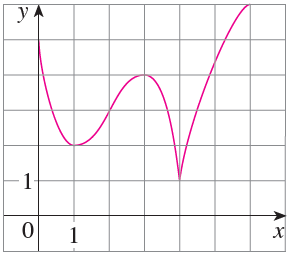
\includegraphics{4.5fig1}
		\end{ex}
			\vs{.5}	
			
		\begin{ex}
			The graph of the \emph{derivative}, \(f'\), is given below.  On what interval(s) is \(f\) increasing or decreasing? At what inputs does \(f\) have a local maximum or minimum?\\
			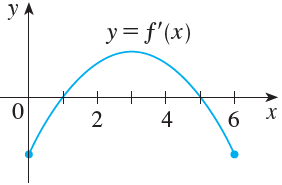
\includegraphics{4.5fig2}
		\end{ex}
			\vs{.5}
		
			\newpage
			
	\subsection*{In Class}
	\subsubsection*{Using Concavity}
		\begin{thm}[Concavity Test]
			If \(f''(x) > 0\) for all \(x\) in \(I\), then the graph of \(f\) is \blank{2} on \(I\).  If \(f''(x) < 0\)\vspace{20pt} for all \(x\) in \(I\), then the graph of \(f\) is \blank{2} on \(I\).
		\end{thm}
		
		\begin{ex}
			Let \(f(x) = x^3 - 3x\).  
			\begin{enumerate}[(a)]
				\item Find the intervals where \(f(x)\) is increasing and decreasing.
					\vs{1}
					
				\item Identify the local maxima and minima of \(f(x)\).
					\vs{.5}
					
				\item Where is \(f\) concave up?  Where is it concave down?
					\vs{1}
					
				\item Identify any inflection points of \(f\).
					\vs{.5}
			\end{enumerate}
		\end{ex}
			\newpage

			
		\begin{thm}[Second Derivative Test]
			Suppose \(f''\) is continuous near \(c\), and \(f'(c) = 0\).  If \blank{1.5}, then \(f\) has a local\vspace{20pt} minimum at \(c\).  If \blank{1.5}, then \(f\) has a local maximum at \(c\).
		\end{thm}

		\begin{ex}
			Find the local maximum and minimum values of \(f(x) = \dfrac{x^2}{x-1}\) using the First and Second Derivative Tests.
		\end{ex}
			\vs{1}
			
		\begin{ex}
			Sketch the curve \(y = x^4-4x^3\) by finding the intervals of increasing/decreasing, local maxima/minima, intervals of concavity, and inflection point(s).
		\end{ex}
			\vs{1}
			\newpage
			
		\begin{ex}
			Sketch the curve \(y=\dfrac{1}{2}x^4 -4x^2 + 3\)
		\end{ex}
			\vs{1}
			
		\begin{ex}
			Sketch the curve \(f(x)=x^3 - 12x + 2\)
		\end{ex}
			\vs{1}
			
		\begin{ex}
			Sketch the curve \(h(x) = 5x^3-3x^5\)
		\end{ex}
			\vs{1}
			\newpage
			
		\begin{ex}
			Sketch the graph of a function that satisfies the criteria outlined below:
				\begin{enumerate}[(i)]
					\item Vertical asymptote at \(x = 0\).
					\item \(f'(x) > 0\) if \(x < -2\), \(f'(x) < 0\) if \(x > -2\) (for \(x\neq 0\)).  
					\item \(f''(x) < 0\) if \(x < 0\), \(f''(x) > 0\) if \(x > 0\).
				\end{enumerate}
		\end{ex}
			\vs{1}
			
		\begin{ex}
			Find all local extrema for \(f(x) = \sqrt[3]{x-1}\).
		\end{ex}
			\vs{1}
			\newpage
			
			

	\subsection*{After Class Practice}
		\begin{ex}
			Find the intervals on which \(\sin x + \cos x\) is increasing/decreasing on \([0,2\pi]\), the local maximum and minimum values of the function on the interval, and the intervals of concavity/inflection points.
		\end{ex}
			\vs{1}
		
		\begin{ex}
			Find the intervals on which \(f(x) = \ln (x\sqrt{x})\) is increasing/decreasing, the local maximum/minimum values of the function, and the intervals of concavity/inflection points. Assume that \(x > 0\).
		\end{ex}	
			\vs{1}
			\newpage
			
		\begin{ex}
			A graph is given below.\\  
			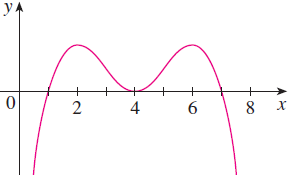
\includegraphics{4.5fig3}\\
			State and justify the \(x-\)coordinates of the inflection points of \(f\), if
			\begin{enumerate}[(a)]
				\item The curve is the graph of\(f\)
					\vs{1}
					
				\item The curve is the graph of \(f'\).
					\vs{1}
					
				\item The curve is the graph of \(f''\).
					\vs{1}
			\end{enumerate}		
		\end{ex}
		
		\begin{ex}
			Consider the phrase ``SAT scores are declining at a slower rate''.  Interpret this statement in terms of a function and its first and second derivatives.
		\end{ex}
			\vs{1}
\clearpage
\end{document}
